\chapter{Návrh}

Tato kapitola popisuje návrh implementace a komplementárních struktur.

\section{Disclosure}

Disclosure je komponenta pro zobrazení a skrývání obsahu.
Typicky se skládá z tlačítka, které otevírá nebo zavírá obsah, a samotného obsahu.

\begin{figure}[htp]
    \centering
    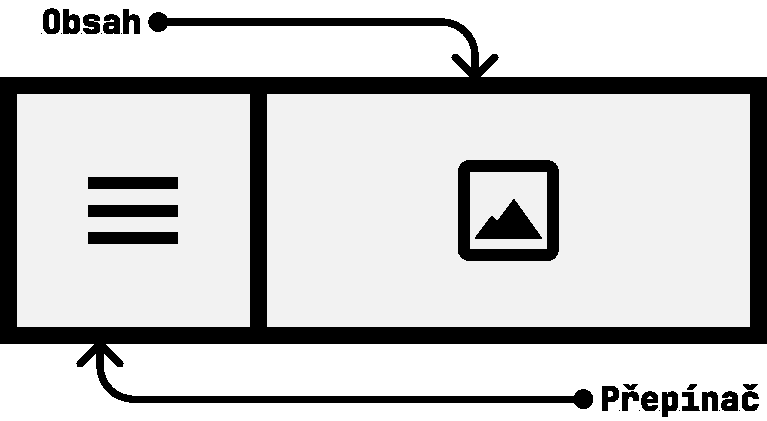
\includegraphics[max size={\linewidth}{\textheight}]{./assets/figures/anatomy/disclosure.pdf}
    \captionsetup{justification=centering}
    \caption[Low-fidelity wireframe komponenty Disclosure]{Low-fidelity wireframe komponenty Disclosure (wireframe autora)}
\end{figure}

Pro splnění požadavku \hyperref[ofr11]{\fr{OFR 1.1}} je potřeba zajistit, že klávesy \keys{\SPACE}, nebo \keys{\enter} mění stav otevření obsahu.

\subsection{Controlled vs Uncontrolled}

Pro splnění požadavku \hyperref[dfr12]{\fr{DFR 1.2}} je potřeba zajistit, že komponenta může být tzv. \textit{controlled} nebo \textit{uncontrolled}.
Většina implementací je ve výchozím režimu uncontrolled, kdy je stav otevření obsahu řízen interním stavem komponenty.
Druhou možností je, aby byla komponenta controlled, kdy je stav otevření obsahu řízen vnějším zdrojem.
V Solid.js je toto řešení implementované pomocí props, kdy z vnějšku komponentě předáme náš vlastní stav, který je následně používaný na místo interního stavu.

\begin{listing}[!ht]
    \begin{minted}{typescript}
const [open, setOpen] = createSignal(false);

const { toggleProps } = createDisclosure({
    isVisible: open,
    onVisibilityChange(state) { setOpen(state) }
});
\end{minted}
    \caption{Ukázka primitivní funkce s vnějším stavem (controlled stav)}
    \label{disclosure-controlled-vs-uncontrolled}
\end{listing}

\section{SpinButton}

SpinButton je formulářová komponenta, která vymezuje rozsah diskrétních hodnot a typicky umožňuje uživateli změnit její hodnotu pomocí tlačítek snížit a navýšit, nebo alternativně skrze textový vstup.

\begin{figure}[htp]
    \centering
    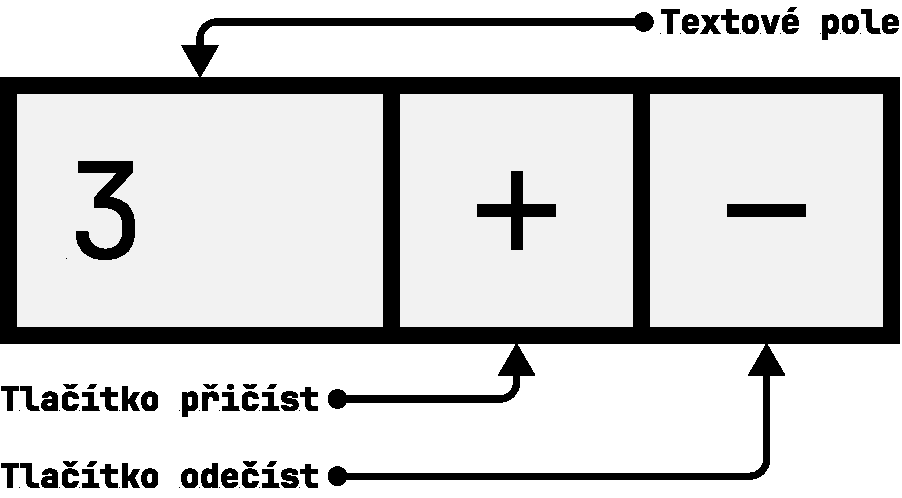
\includegraphics[max size={\linewidth}{\textheight}]{./assets/figures/anatomy/spinbutton.pdf}
    \captionsetup{justification=centering}
    \caption[Low-fidelity wireframe komponenty SpinButton]{Low-fidelity wireframe komponenty SpinButton (wireframe autora)}
\end{figure}

Pro splnění požadavku \hyperref[ofr11]{\fr{OFR 1.1}} a \hyperref[sfr12]{\fr{SFR 1.2}} je potřeba splnit následující podmínky:

\begin{enumerate}
    \item Klávesové šipky \keys{\arrowkeyup} a \keys{\arrowkeydown} zvýší, respektive sníží hodnotu o jedna.
    \item Klávesy \keys{PageUp} a \keys{PageDown} zvýší, respektive sníží hodnotu o vybraný krok.
    \item Klávesy \keys{Home} a \keys{End} nastaví hodnotu na minimum, respektive maximum.
\end{enumerate}

\section{Toolbar}

Toolbar je strukturální komponenta, která obsahuje skupinu focusovatelných elementů.

\begin{figure}[htp]
    \centering
    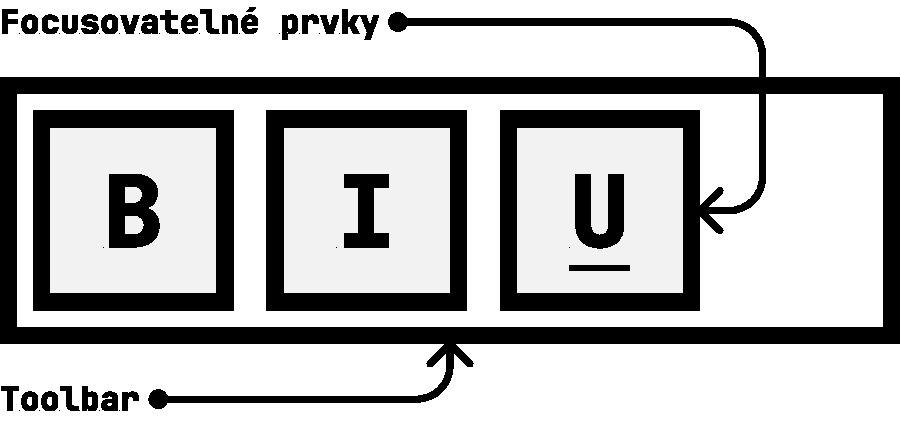
\includegraphics[max size={\linewidth}{\textheight}]{./assets/figures/anatomy/toolbar.pdf}
    \captionsetup{justification=centering}
    \caption[Low-fidelity wireframe komponenty Toolbar]{Low-fidelity wireframe komponenty Toolbar (wireframe autora)}
\end{figure}

Hlavní přínos této komponenty je jednodušší klávesová navigace pomocí klávesových šipek a dalších zkratek namísto klasického proklikávání tabulátorem.

Pro splnění požadavku \hyperref[ofr11]{\fr{OFR 1.1}} je potřeba splnit následující podmínky:

\begin{enumerate}
    \item Klávesa \keys{\tab} (tab), nebo klávesová zkratka \keys{\tab + \shift} skočí na první, nebo naposled vybraný focusovatelný prvek v rámci Toolbaru.
    \item Klávesa \keys{\tab}, když je focus v rámci Toolbaru, skočí na první focusovatelný prvek mimo Toolbar, který se nachází v hierarchii za Toolbar komponentou.
    \item Klávesová zkratka \keys{\tab + \shift}, když je focus v rámci Toolbaru, skočí na první focusovatelný prvek mimo Toolbar, který se nachází v hierarchii před Toolbar komponentou.
    \item Klávesové šipky \keys{\arrowkeyleft} a \keys{\arrowkeyright} přesunou focus mezi focusovatelnými prvky v rámci Toolbaru pokud je orientace toolbaru horizontální.
    \item Klávesové šipky \keys{\arrowkeyup} a \keys{\arrowkeydown} přesunou focus mezi focusovatelnými prvky v rámci Toolbaru pokud je orientace toolbaru vertikální.
    \item Klávesy \keys{Home} a \keys{End} přesunou focus na první, respektive poslední focusovatelný prvek v rámci Toolbaru.
\end{enumerate}

\section{Tooltip}

Tooltip je komponenta, která zobrazí nápovědu u vybraného elementu (nejčastěji se bude jednat o interaktivní element) po najetí myši, nebo při předání focusu na daný element (viz funkční požadavek \hyperref[tlfr11]{\fr{TLFR 1.1}}).

\begin{figure}[htp]
    \centering
    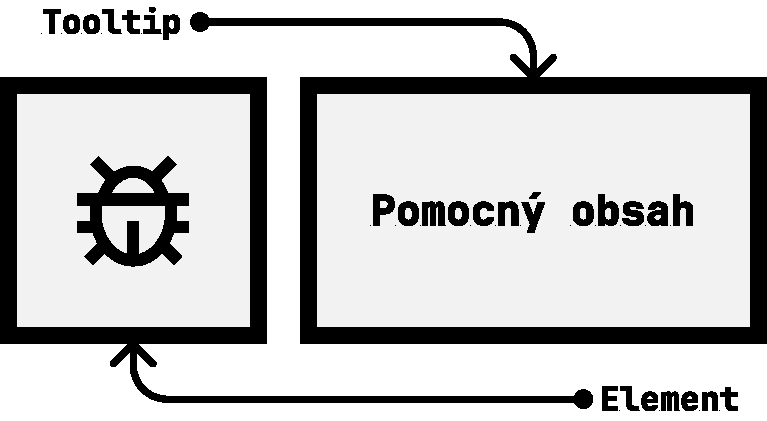
\includegraphics[max size={\linewidth}{\textheight}]{./assets/figures/anatomy/tooltip.pdf}
    \captionsetup{justification=centering}
    \caption[Low-fidelity wireframe komponenty Tooltip]{Low-fidelity wireframe komponenty Tooltip (wireframe autora)}
\end{figure}

Pro splnění požadavku \hyperref[ofr11]{\fr{OFR 1.1}} je potřeba zajistit jedinou klávesovou interakci pomocí klávesy \keys{\esc}, která uzavře obsah pokud je zobrazený.

\clearpage

\section{Dokumentace}

Součástí zadání práce a požadavku \hyperref[nfr14]{\fr{NFR 1.4}} je vytvoření dokumentace pro implementované komponenty.
Dokumentace by měla obsahovat několik zásadních sekcí:

\begin{enumerate}
    \item \textbf{Anatomie komponenty}

          Anatomie by měla popisovat způsob naimportování knihovny, její typovou signaturu a low-fidelity návrh.

    \item \textbf{API reference}

          \gls{api} reference by měla popisovat vstupní parametry, jejich výchozí hodnoty a typ tak, aby ušetřila čas vývojáři pro pochopení implementace.

    \item \textbf{Příklad}

          Příklad by měl být vnořený na stránce tak, aby komponentu šlo používat jako v normální aplikaci. Součástí příkladu by měl být kopírovatelný zdrojový kód.

    \item \textbf{Ukázka s odečítačem obrazovky}

          V dokumentaci by měla být i ukázka toho, jak komponenta reaguje na použití s odečítačem obrazovky.

\end{enumerate}

Kromě výše zmíněných částí u každé stránky s komponentou by měla dokumentace obsahovat informace o tom, jak knihovnu nainstalovat a které technologie je potřeba mít nainstalované.
V neposlední řadě by měla dokumentace obsahovat odkazy na informaci o implementovaném návrhovém vzoru, výsledky testů a pokrytí kódu testy.

\clearpage

\subsection{Diagram obrazovek}

Na obrázku~\ref{figure:screenmap} je diagram obrazovek dokumentace, který i nepřímo popisuje komponentovou strukturu dokumentace.
Nejdůležitější částí je sekce \texttt{Primitives}, která obsahuje stránky dokumentující každou implementovanou komponentu.

\begin{figure}[htp]
    \centering
    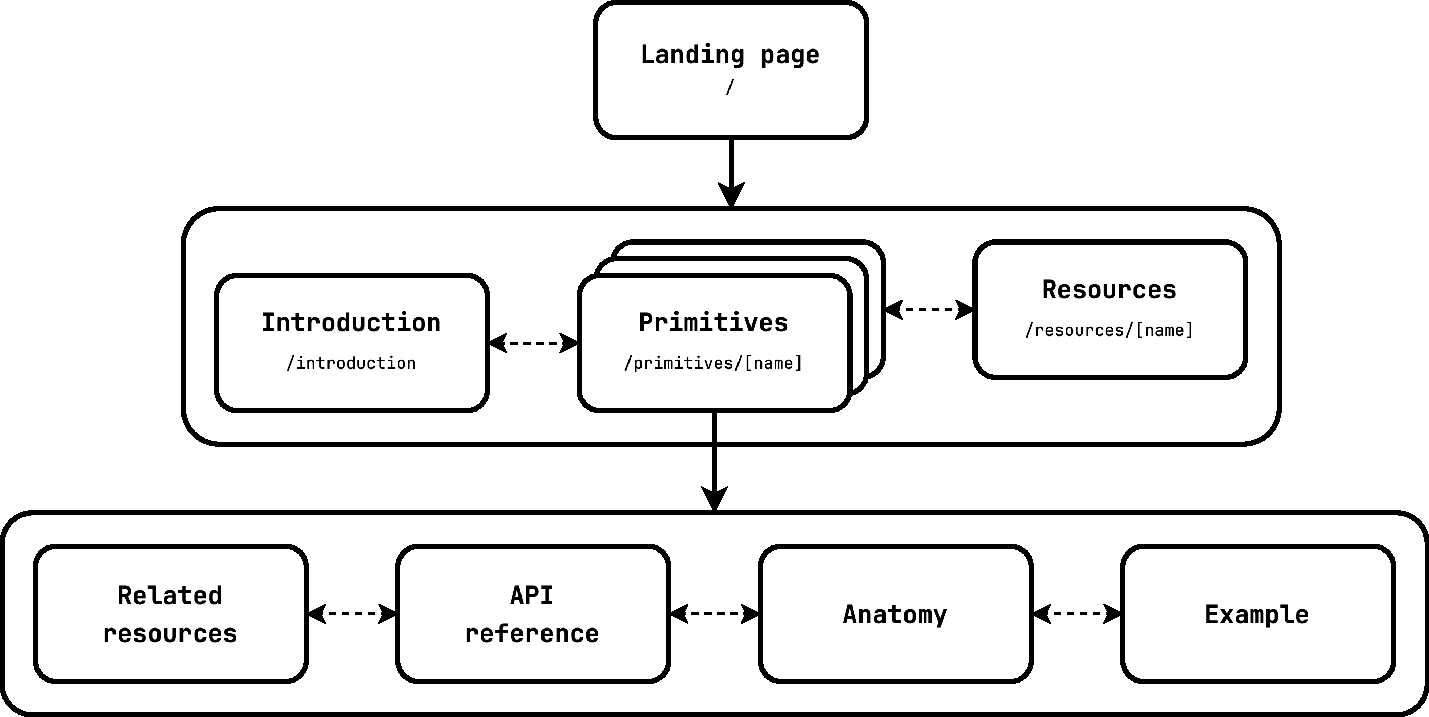
\includegraphics[max size={\linewidth}{\textheight}]{./assets/figures/screenmap.pdf}
    \captionsetup{justification=centering}
    \caption[Diagram obrazovek dokumentace]{Diagram obrazovek dokumentace (diagram autora)}
    \label{figure:screenmap}
\end{figure}
